% A LaTeX template for EXECUTIVE SUMMARY of the MSc Thesis submissions to 
% Politecnico di Milano (PoliMi) - School of Industrial and Information Engineering
%
% https://www.ingindinf.polimi.it/it/didattica/lezioni-e-esami/esami-di-laurea-e-laurea-magistrale
%
% S. Bonetti, A. Gruttadauria, G. Mescolini, A. Zingaro
% e-mail: template-tesi-ingind@polimi.it
%
% Last Revision: October 2021
%
% Copyright 2021 Politecnico di Milano, Italy. NC-BY

\documentclass[11pt,a4paper,twocolumn]{article}

%------------------------------------------------------------------------------
%	REQUIRED PACKAGES AND  CONFIGURATIONS
%------------------------------------------------------------------------------
% PACKAGES FOR TITLES
\usepackage{titlesec}
\usepackage{color}

% PACKAGES FOR LANGUAGE AND FONT
\usepackage[utf8]{inputenc}
\usepackage[english]{babel}
\usepackage[T1]{fontenc} % Font encoding

% PACKAGES FOR IMAGES
\usepackage{graphicx}
\graphicspath{{Images/}} % Path for images' folder
\usepackage{eso-pic} % For the background picture on the title page
\usepackage{subfig} % Numbered and caption subfigures using \subfloat
\usepackage{caption} % Coloured captions
\usepackage{transparent}

% STANDARD MATH PACKAGES
\usepackage{amsmath}
\usepackage{amsthm}
\usepackage{bm}
\usepackage[overload]{empheq}  % For braced-style systems of equations

% PACKAGES FOR TABLES
\usepackage{tabularx}
\usepackage{longtable} % tables that can span several pages
\usepackage{colortbl}

% PACKAGES FOR ALGORITHMS (PSEUDO-CODE)
\usepackage{algorithm}
\usepackage{algorithmic}

% PACKAGES FOR REFERENCES & BIBLIOGRAPHY
\usepackage[colorlinks=true,linkcolor=black,anchorcolor=black,citecolor=black,filecolor=black,menucolor=black,runcolor=black,urlcolor=black]{hyperref} % Adds clickable links at references
\usepackage{cleveref}
\usepackage[square, numbers, sort&compress]{natbib} % Square brackets, citing references with numbers, citations sorted by appearance in the text and compressed
\bibliographystyle{plain} % You may use a different style adapted to your field

% PACKAGES FOR THE APPENDIX
\usepackage{appendix}

% PACKAGES FOR ITEMIZE & ENUMERATES 
\usepackage{enumitem}

% OTHER PACKAGES
\usepackage{amsthm,thmtools,xcolor} % Coloured "Theorem"
\usepackage{comment} % Comment part of code
\usepackage{fancyhdr} % Fancy headers and footers
\usepackage{lipsum} % Insert dummy text
\usepackage{tcolorbox} % Create coloured boxes (e.g. the one for the key-words)
\usepackage{stfloats} % Correct position of the tables

%-------------------------------------------------------------------------
%	NEW COMMANDS DEFINED
%-------------------------------------------------------------------------
% EXAMPLES OF NEW COMMANDS -> here you see how to define new commands
\newcommand{\bea}{\begin{eqnarray}} % Shortcut for equation arrays
\newcommand{\eea}{\end{eqnarray}}
\newcommand{\e}[1]{\times 10^{#1}}  % Powers of 10 notation
\newcommand{\mathbbm}[1]{\text{\usefont{U}{bbm}{m}{n}#1}} % From mathbbm.sty
\newcommand{\pdev}[2]{\frac{\partial#1}{\partial#2}}
% NB: you can also override some existing commands with the keyword \renewcommand

%----------------------------------------------------------------------------
%	ADD YOUR PACKAGES (be careful of package interaction)
%----------------------------------------------------------------------------


%----------------------------------------------------------------------------
%	ADD YOUR DEFINITIONS AND COMMANDS (be careful of existing commands)
%----------------------------------------------------------------------------


% Do not change Configuration_files/config.tex file unless you really know what you are doing. 
% This file ends the configuration procedures (e.g. customizing commands, definition of new commands)
% Set the geometric layout of the document
\usepackage{geometry}
\geometry{
  top=2.8cm,
  left = 1.9cm,
  right = 1.9cm,
  bottom=2.0cm,
  headheight= 2cm,
  headsep= 0cm,
}
\raggedbottom 

% Create color bluePoli (-> manuale grafica coordinata:  https://www.polimi.it/fileadmin/user_upload/il_Politecnico/grafica-coordinata/2015_05_11_46xy_manuale_grafica_coordinata.pdf)
\definecolor{bluePoli}{cmyk}{0.4,0.1,0,0.4}

% Custom theorem environments
\declaretheoremstyle[
  headfont=\color{bluePoli}\normalfont\bfseries,
  bodyfont=\color{black}\normalfont\itshape,
]{colored}

\captionsetup[figure]{labelfont={color=bluePoli}} % Set colour of the captions
\captionsetup[table]{labelfont={color=bluePoli}} % Set colour of the captions
\captionsetup[algorithm]{labelfont={color=bluePoli}} % Set colour of the captions

\theoremstyle{colored}
\newtheorem{theorem}{Theorem}[section]
\newtheorem{proposition}{Proposition}[section]

% Enhances the features of the standard "table" and "tabular" environments.
\newcommand\T{\rule{0pt}{2.6ex}}
\newcommand\B{\rule[-1.2ex]{0pt}{0pt}}

% Algorithm description
\newcounter{algsubstate}
\renewcommand{\thealgsubstate}{\alph{algsubstate}}
\newenvironment{algsubstates}{
    \setcounter{algsubstate}{0}%
    \renewcommand{\STATE}{%
    \stepcounter{algsubstate}%
    \Statex {\small\thealgsubstate:}\space}
    }{}
    
% Custom theorem environment
\newcolumntype{L}[1]{>{\raggedright\let\newline\\\arraybackslash\hspace{0pt}}m{#1}}
\newcolumntype{C}[1]{>{\centering\let\newline\\\arraybackslash\hspace{0pt}}m{#1}}
\newcolumntype{R}[1]{>{\raggedleft\let\newline\\\arraybackslash\hspace{0pt}}m{#1}}

% Custom itemize environment
\setlist[itemize,1]{label=$\bullet$}
\setlist[itemize,2]{label=$\circ$}
\setlist[itemize,3]{label=$-$}
\setlist{nosep}

% Set separation of columns 
\setlength{\columnsep}{30pt}

% Create command for background pic
\newcommand\BackgroundPic{% Adding background picture
	\put(237,365){
		\parbox[b][\paperheight]{\paperwidth}{%
			\vfill
			\centering
			\transparent{0.4}
			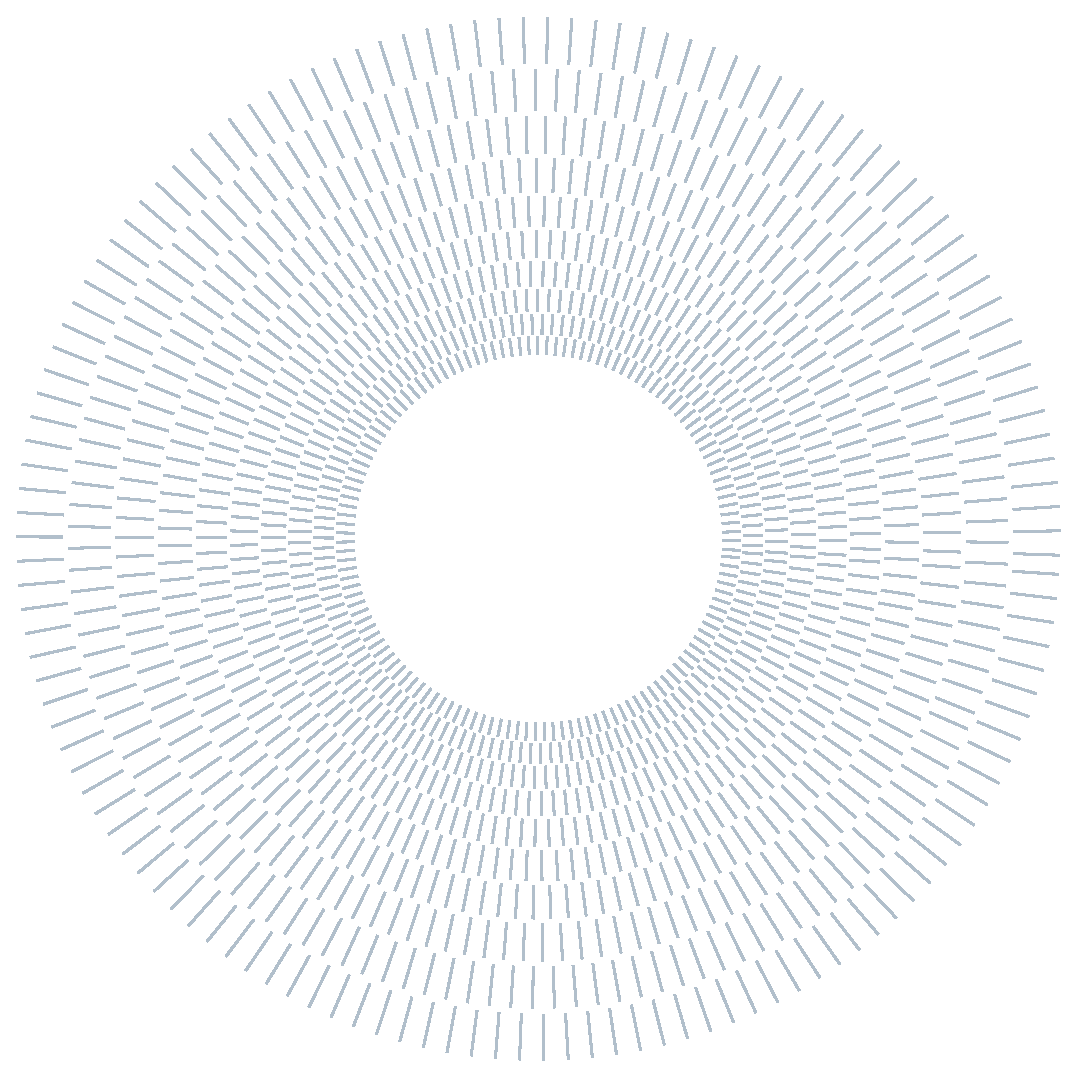
\includegraphics[width=0.44\paperwidth]{raggiera_polimi.eps}%
			\vfill
}}}

% Set indentation
\setlength\parindent{0pt}

% Custom title commands
\titleformat{\section}
{\color{bluePoli}\normalfont\Large\bfseries}
{\color{bluePoli}\thesection.}{1em}{}
\titlespacing*{\section}
{0pt}{2ex}{1ex}

\titleformat{\subsection}
{\color{bluePoli}\normalfont\large\bfseries}
{\color{bluePoli}\thesubsection.}{1em}{}
\titlespacing*{\subsection}
{0pt}{2ex}{1ex}

% Custom headers and footers
\pagestyle{fancy}
\fancyhf{}
      
\fancyfoot{}
\fancyfoot[C]{\thepage} % page
\renewcommand{\headrulewidth}{0mm} % headrule width
\renewcommand{\footrulewidth}{0mm} % footrule width

\makeatletter
\patchcmd{\headrule}{\hrule}{\color{black}\hrule}{}{} % headrule
\patchcmd{\footrule}{\hrule}{\color{black}\hrule}{}{} % footrule
\makeatother

% -> Create the header
\chead[C]{
\centering
\begin{tcolorbox}[arc=0pt, boxrule=0pt, colback=bluePoli!60, width=\textwidth, colupper=white, top=1.7mm, bottom=1.7mm]
    \textbf{Executive summary} \hfill \textbf{\author}  
\end{tcolorbox}
}

% Insert here the info that will be displayed into your Title page 
% -> title of your work
\renewcommand{\title}{Location-Aware and Stateful Serverless Computing on the Edge}
% -> author name and surname
\renewcommand{\author}{Dennis Motta}
% -> MSc course
\newcommand{\course}{Computer Science and Engineering}
% -> advisor name and surname
\newcommand{\advisor}{Alessandro Margara}
% IF AND ONLY IF you need to modify the co-supervisors you also have to modify the file Configuration_files/title_page.tex (ONLY where it is marked)
\newcommand{\firstcoadvisor}{Gianpaolo Cugola} % insert if any otherwise comment
%\newcommand{\secondcoadvisor}{Name Surname} % insert if any otherwise comment
% -> academic year
\newcommand{\YEAR}{2020-2021}

%-------------------------------------------------------------------------
%	BEGIN OF YOUR DOCUMENT
%-------------------------------------------------------------------------
\begin{document}

%-----------------------------------------------------------------------------
% TITLE PAGE
%-----------------------------------------------------------------------------
% Do not change Configuration_files/TitlePage.tex (Modify it IF AND ONLY IF you need to add or delete the Co-advisors)
% This file creates the Title Page of the document
% DO NOT REMOVE SPACES BETWEEN LINES!

\twocolumn[{\begin{@twocolumnfalse}

\AddToShipoutPicture*{\BackgroundPic}

\hspace{-0.6cm}
\includegraphics[width=0.6\textwidth]{logo_polimi_ing_indinf.eps}

\vspace{-1mm}
\fontsize{0.3cm}{0.5cm}\selectfont \bfseries \textsc{\color{bluePoli} Executive Summary of the Thesis}\\

\vspace{-0.2cm}
\Large{\textbf{\color{bluePoli}{\title}}}\\

\vspace{-0.2cm}
\fontsize{0.3cm}{0.5cm}\selectfont \bfseries \textsc{\color{bluePoli} Master of Science in \course}\\

\vspace{-0.2cm}
\fontsize{0.3cm}{0.5cm} \selectfont \bfseries Author: \textsc{\textbf{\author}}\\

\vspace{-0.4cm}
\fontsize{0.3cm}{0.5cm}\selectfont \bfseries Advisor: \textsc{\textbf{\advisor}}\\

% if only ONE co-advisor is present:
\vspace{-0.4cm}
\fontsize{0.3cm}{0.5cm}\selectfont \bfseries Co-advisor: \textsc{\textbf{\firstcoadvisor}}\\
% if more than one co-advisors are present:
%\vspace{-0.4cm}
%\fontsize{0.3cm}{0.5cm}\selectfont \bfseries Co-advisors: \textsc{\textbf{\firstcoadvisor}}\textsc{\textbf{\secondcoadvisor}}\\

\vspace{-0.4cm}
\fontsize{0.3cm}{0.5cm}\selectfont \bfseries Academic year: \textsc{\textbf{\YEAR}}

\small \normalfont

\vspace{11pt}

\centerline{\rule{1.0\textwidth}{0.4pt}}

\vspace{15pt}
\end{@twocolumnfalse}}]

\thispagestyle{plain} % In order to not show the header in the first page

%%%%%%%%%%%%%%%%%%%%%%%%%%%%%%
%%     THESIS MAIN TEXT     %%
%%%%%%%%%%%%%%%%%%%%%%%%%%%%%%

%-----------------------------------------------------------------------------
% CONTENT
%-----------------------------------------------------------------------------
\chapter{Introduction}

\section{Context}

% This is basically an extension of the abstract. Here you provide context for the problem faced. Keep in mind that even if you now have gained expertise on it, most of the readers are no so inside the problem as you are. Start from the basics and explain clearly. You can also introduce here some hints about the methodology and your contribution. For this purpose, you may also decide to add more sections.

With the increasing number of connected devices and with Internet-of-Thing (IoT) implementation now becoming more widespread, in some cases cloud-centric architectures are starting to be ineffective. Devices are generating a lot of data at the end of the network and many applications are already being deployed at the edge to process the information.
Cisco Systems predicts that an estimated 29 billion devices will connect to the Internet by 2023 \cite{cisco2018-2023}.

Due to the volume, variety and velocity of data generated at the end of the network, the cloud cannot fully support applications that must meet compelling \textbf{latency} or \textbf{bandwidth} constraints: huge distances need to be covered by the communication, increasing the latency and making a large quantity of data pass through the network.
Indeed, the considerable increase in the amount of data produced at the end of the network was not accompanied by a comparable increase of available bandwidth from/to the cloud \cite{promise-of-edge-computing}.

% Furthermore, Cloud connection latencies are not adequate to host real-time tasks such as life-saving connected devices, augmented reality, or gaming [3].

% Some of the applications they run might require very short response times, some might involve private data, and some might produce huge quantities of data. Cloud computing can’t support these IoT applications. Edge computing, on the other hand, can do so and will promote many new IoT applications.

\section{Research Questions}
An increasing trend in edge computing has been found in the last years, however the industry lacks the presence of a development abstraction with stateful support that allows developers to easily exploit the power of the edge. The absence of this abstraction makes developers still prefer cloud-centric approaches despite the related problems.

A non-technology and non-infrastructure dependant framework is needed in order to allow the development of applications with strict constraints of latency and bandwidth.

Therefore this work aims at answering the following research questions (RQ):
\begin{itemize}
    \item[\textit{RQ.1}]\emph{Which use cases are predominantly affected by bandwidth and latency constraints? What are the common characteristics of these use cases?}
    
    \item[\textit{RQ.2}]\emph{Which frameworks allowing computation on the edge are currently available in the industry? Can the available frameworks accomplish the use cases seen in RQ.1?}
    
    \item[\textit{RQ.3}]\emph{Can a new approach accomplish the use cases seen in RQ.1? How can such approach be implemented?}
    
    \item[\textit{RQ.4}]\emph{Does the new approach simplify the development? Is it easy to use?}
    
    \item[\textit{RQ.5}]\emph{Does the new approach obtain better performance? What are the practical measurable benefits? How much resources does it use? What are its drawbacks?}
\end{itemize}

We use the answers to these questions to propose an innovative framework that allows the developers to abstract away both the infrastructure and the location of the users.

\section{Research Methodology}
The research approach adopted in this thesis can be summarized at high-level with the following steps:
\begin{itemize}
    \item A review and analysis of the \textbf{state‐of‐the‐art} research on edge and fog computing, with a particular emphasis on \textbf{data processing} and identification of objectives;
    
    \item Identification of common \textbf{use cases} and formulation of the key requirements needed to better fulfill the use cases;
    
    \item A review of the publicly \textbf{available frameworks} provided by the industry in the field of edge computing, stateful logic on the edge and Function-as-a-Service (FaaS). 
    
    \item Design of a novel problem \textbf{solution} based on the identified requirements;
    
    \item \textbf{Evaluation} of the solution through the development of a prototype and through simulations.
\end{itemize}
A thorough literature review is the basis of this thesis. For this purpose, we do not limit the analysis scope to the edge data processing problem and instead enlarge our focus generally to edge and fog computing. We started from surveys on edge computing, then moved to papers presented at the "IEEE International Conference on Fog and Edge Computing (ICFEC)", especially focusing on papers about data processing, and finally we performed specific searches to have a deeper emphasis on the data processing part.
We gained understanding of the main issues and collected the motivating use cases (\textit{RQ.1}).

We then moved to a review of publicly available frameworks provided by the industry and analyzed their usability in relation with the motivating use cases collected (\textit{RQ.2}). As we will show we did not find any framework able to sufficiently fulfill the use cases, so we tried to propose a novel solution.

To analyze the effectiveness of our solution we implemented a working prototype (\textit{RQ.3}) and by using our implementation we were able to study its value and benefits (\textit{RQ.4}). Due to the size of an edge network, emulating our prototype to study its performance on a similar setup was infeasible, so we developed a discrete-event simulation to simulate the behavior of our approach in a scenario more similar to the real (\textit{RQ.5}).

The \textbf{resulting artifacts} of our research have been released as open-source software \cite{thesis-github}.


\section{Thesis Outline}
The remainder of this thesis is organized as follows.

In Chapter \ref{ch:preliminaries_and_open_problems}, we review and analyze \textbf{state-of-the-art} solutions in the field of Edge Computing, starting from surveys and general concepts and then moving our focus to the data processing part. We then define the \textbf{open problems} by collecting, organizing and commenting the \textbf{use cases} which we have encountered in our research.

In Chapter \ref{ch:existing-solutions}, we present the solutions made available publicly by the industry in the field of Edge Computing. We show that the \textbf{current solutions} do not cover in an adequate way the use cases collected.

In Chapter \ref{ch:design-of-the-solution}, we develop the idea of \textbf{our solution}, showcasing the intended usage of our APIs.

In Chapter \ref{ch:prototype}, we show our actual \textbf{implementation} of the solution we proposed.

In Chapter \ref{ch:evaluation}, we investigate the \textbf{gains} developers may obtain by using our approach and we demonstrate how several use cases can benefit from this new system though discrete-event simulation.

We \textbf{conclude} in Chapter \ref{ch:conclusions}, summarizing our contributions and highlighting possible future research directions.


\section{Guidelines}
\label{sec:guidelines}

The Executive Summary is a critical overview of your thesis
with a focus on the main achievements that have emerged from your research.

The Executive Summary should be organized in sections/paragraphs
in order to better highlight the major points of your work.
The length should range from four to six pages depending on the length of the thesis manuscript.
Keep the Executive Summary concise enough to be effective but long enough to allow it to be complete.
It should be written after completing the thesis manuscript as a stand-alone independent document
of sufficient clarity and detail to ensure that the reader can figure out the overall objectives,
the methodology employed and the results/impact of your research.

In writing the Executive Summary, keep in mind that it is not an abstract, it is not a preface,
and it is not a random collection of highlights.
With a few exceptions, do not simply cut and paste whole sections or paragraphs of the thesis manuscript
into a disorganized and cluttered Executive Summary.
You should reorganize information to be informative as well as concise.

The Executive Summary could contain a few important equations related to your work.
It could also include the most relevant figures and tables taken or elaborated from the thesis manuscript.

You should also include in the Executive Summary the very essential bibliography of your study.
The number of selected references should range from three to five depending on the type of work.

The Executive Summary should contain a final section reporting the main conclusions drawn from your research.

\section{Sections and subsections}
\label{sec:sec_and_subsec}
It is convenient to organize the Executive Summary of your thesis into sections and subsections. 
If necessary, subsubsections, paragraphs and subparagraphs can be also used. 
A new section or subsection can be included  with the commands
\begin{verbatim}
\section{Title of the section}
\end{verbatim}
\begin{verbatim}
\subsection{Title of the subsection}
\end{verbatim}
It is recommended to give a label to each section by using the command
\begin{verbatim}
\label{sec:section_name}%
\end{verbatim}
where the argument is just a text string that you'll use to reference that part
as follows: \textit{Section~\ref{sec:sec_and_subsec} contains \sc{SECTIONS AND SUBSECTIONS}  \dots}.

\section{Equations, Figures, Tables and Algorithms}
\label{sec:equations_and_figures}
All Figures, Tables and Algorithms have to be properly referred in the text.
Equations have to be numbered only if they are referred in the text.
\subsection{Equations}
\label{sec_equations}
A few important equations related to your work might be reported in the Executive Summary. For example, the Maxwell's equations read:
\begin{subequations}
    \label{eq:maxwell}
    \begin{align}[left=\empheqlbrace]
    \nabla\cdot \bm{D} & = \rho, \label{eq:maxwell1} \\
    \nabla \times \bm{E} +  \frac{\partial \bm{B}}{\partial t} & = \bm{0}, \label{eq:maxwell2} \\
    \nabla\cdot \bm{B} & = 0, \label{eq:maxwell3} \\
    \nabla \times \bm{H} - \frac{\partial \bm{D}}{\partial t} &= \bm{J}. \label{eq:maxwell4}
    \end{align}
\end{subequations}

Equation~\eqref{eq:maxwell} is automatically labeled by \texttt{cleveref},
as well as Equation~\eqref{eq:maxwell1} and Equation~\eqref{eq:maxwell3}.
Thanks to the \verb|cleveref| package, there is no need to use \verb|\eqref|.

\subsection{Figures}
\label{sec:figures}
To include Figures in your text you can use \texttt{TikZ} for high-quality hand-made figures \cite{tikz},
or just include them with the command
\begin{verbatim}
\includegraphics[options]{filename.xxx}
\end{verbatim}
where xxx is the format (\verb|.png|, \verb|.jpg|, \verb|.eps|, \dots).
An example is shown in Figure~\ref{fig:quadtree}.
\begin{figure}[H]
    \centering
    
\includegraphics[width=0.3\textwidth]{logo_polimi_scritta.eps}
    \caption{Caption of the Figure.}
    \label{fig:quadtree}
\end{figure}

\subsection{Tables}
\label{subsec:tables}

Within the environments \texttt{table} and  \texttt{tabular} you can create very fancy tables like the one shown in Table~\ref{table:example}.
\begin{table}[H]
    \caption*{\textbf{Example of Table}}
    \centering 
    \begin{tabular}{|p{3em} c c c |}
    \hline
    \rowcolor{bluePoli!40}
     & \textbf{column1} & \textbf{column2} & \textbf{column3} \T\B \\
    \hline \hline
    \textbf{row1} & 1 & 2 & 3 \T\B \\
    \textbf{row2} & $\alpha$ & $\beta$ & $\gamma$ \T\B\\
    \textbf{row3} & alpha & beta & gamma \B\\
    \hline
    \end{tabular}
    \\[10pt]
    \caption{Caption of the Table.}
    \label{table:example}
\end{table}

\subsection{Algorithms}
\label{subsec:algorithms}

Pseudo-algorithms can be written in \LaTeX{} with the \texttt{algorithm} and \texttt{algorithmic} packages.
One example follows.
\begin{algorithm}[H]
\label{alg:example}
\caption{Name of the Algorithm}
\label{alg:var}
\label{protocol1}
\begin{algorithmic}[1]
\STATE Initial instructions
\FOR{$for-condition$}
\STATE{Some instructions}
\IF{$if-condition$}
\STATE{Some other instructions}
\ENDIF
\ENDFOR
\WHILE{$while-condition$}
\STATE{Some further instructions}
\ENDWHILE
\STATE Final instructions
\end{algorithmic}
\end{algorithm} 

\section{Some further useful recommendations}

Theorems and Propositions have to be formatted as follows:
\begin{theorem}
\label{a_theorem}
Write here your theorem. 
\end{theorem}
\textit{Proof.} If useful you can report here the proof.
\vspace{0.3cm} % Insert vertical space

How to write propositions:
\begin{proposition}
Write here your proposition.
\end{proposition}
\vspace{0.3cm} % Insert vertical space

How to insert itemized lists:
\begin{itemize}
    \item first item;
    \item second item.
\end{itemize}
How to insert numbered lists:
\begin{enumerate}
    \item first item;
    \item second item.
\end{enumerate}

\section{Bibliography}
\label{sec:bibliography}
The Executive Summary should contain the very essential bibliography of your study.
It is suggested to use the BibTeX package \cite{bibtex} and save the bibliographic references
in the file  \verb|bibliography.bib|.

\chapter{Conclusions and Future Developments}
\label{ch:conclusions}


\section{Conclusions}
The large diffusion of smart devices and IoT sensors has resulted in an \textbf{unprecedented growth} in the amount of collected data. Core-centric approaches have shown to be inefficient as they need to transfer data back and forth between the core and the devices, generating notable latencies. Therefore new approaches, which exploit the \textbf{tremendous power of the edge} of the network, are replacing the core-centric approaches.

In this thesis we have studied the problem of performing \textbf{stateful computations in a geo-distributed and heterogeneous scenario}, that is the edge of the network.

After analyzing the state of the art in the literature, we defined key research questions that guided our research.
We started by \textbf{collecting and organizing the use cases} predominantly affected by bandwidth and latency constraints. With the use cases at hand we \textbf{studied the current frameworks} provided by the industry and we noticed that some of the use cases were left out and couldn't be fulfilled by the available frameworks. This situation forces developers to create ad hoc solutions on the infrastructure, a process which is error-prone and task-specific.

Therefore we tried to solve the gap of fulfillment present in the use cases, by proposing a \textbf{new solution} which supports the characteristics of the use cases left out. We designed and then implemented a \textbf{prototype} for this solution which brings stateful computations and location awareness in contexts where a change of location of the clients does not occur or is not important (the solution in fact does not provide session consistency).

We then \textbf{evaluated} the performance and usability of our prototype in a simple scenario. Instead to evaluate the solution in a complex but more realistic scenario we resorted to a \textbf{discrete-event simulation}.
We found that, by using our framework with the right use cases, we get immense benefits in terms of \textbf{reduced traffic} in the network and in terms of \textbf{lower latencies}, especially in cases where the data aggregation needed is not central. However we also noticed how our solution can be affected by a latency increase due to random spikes in the requests and due to the small number of cores and resources at the edge of the network. Nevertheless the results of the evaluation confirmed the \textbf{power and effectiveness of the proposed solution}.


\section{Future Developments}
In this thesis, we have addressed several key issues related to stateful serverless computing on the edge by designing and implementing a new solution. However, with our solution, not every use case can be fulfilled, in fact the absence of \textbf{session consistency} makes the usage impractical in a dynamic context where the location of the client changes.
Therefore a possible improvement and a possible research direction could be session consistency in the context of stateful serverless computing on the edge.

Another problem with our solution is the possibility for edge locations to be overwhelmed due to random spikes in requests targeting a specific location: our solution does not support the \textbf{offload of the computation} to free up some resources from an overloaded node. On the contrary, for how we thought our solution, in some use cases it's important to be static and to always reach the same node. 

In the context of serverless computing a common problem is the phenomenon of \textbf{cold-start}, which impacts processing latency. As we saw, there exist solutions that firmly mitigated the problem reaching milliseconds cold-start latencies (Cloudflare Workers), but unfortunately these solutions are currently proprietary.

\section{Acknowledgements}
Here you might want to acknowledge someone.


%---------------------------------------------------------------------------
%  BIBLIOGRAPHY
%---------------------------------------------------------------------------
% Remember to insert here only the essential bibliography of your work
\bibliography{bibliography.bib} % automatically inserted and ordered with this command 

\end{document}